%\graphicspath{{/home/arbon/Pictures/Screenshots/}} % path to graphics
\graphicspath{{~/Documents/SADT/SecondTask/img/}}
\chapter*{\LARGE{Цель практической работы}}
\addcontentsline{toc}{chapter}{Цель практической работы}
Данная практическая работа посвящена написанию базовых bash-скриптов.

По сути своей Bash-скриптов представляют из себя ни что иное как
последовательность команд командной строки, объединенных в один файл
для решения какой-либо задачи.

\chapter{Bash}
\section{Базовые Bash скрипты}
\paragraph{Cценарий, который выводит дату, время, список
зарегистрировавшихся пользователей, и uptime системы и сохраняет
эту информацию в файл}\mbox{}\par
Данный сценарий принемает параметром имя файла в который будет сохранятся
информация. Сам сценарий будет состоять из четырех команд:
\begin{itemize}
	\item \texttt{data} - выводит текущую дату и время;
	\item \texttt{cat} - выводит содержимое файла переданного ей параметром.
		В скрипте параметром передается файл \texttt{/etc/passwd},
		где храниться список всех пользователей;
	\item \texttt{cut} - обрезает строки, переданные ей на вход;
	\item \texttt{uptime} - возвращает информацию как долго система
		была запущена.
\end{itemize}
Код скрипта показан в листнинге \ref{lst:date}.

\begin{lstlisting}[language=Bash
	, caption=\leftline{Код скрипта}
	, label=lst:date]
#!/bin/sh
date > "\$1"
cat /etc/passwd | cut -d':' -f 1 >> "\$1"
uptime >> "\$1"
echo "" >> "\$1"
\end{lstlisting}

\paragraph{Cценарий, который выводит содержимое любого каталога
или сообщение о том, что его не существует}\mbox{}\par
Для реализации данного скрипта используется управляющая конструкция
\texttt{if-then-else}. В условии используется команда \texttt{test},
ее сокращенная форма с квадратными скобками, и флаг \texttt{-d}
для проверки файла, является ли он директорией.\par
Код скрипта показан в листнинге \ref{lst:chdir}.

\begin{lstlisting}[language=Bash
	, caption=\leftline{Проверка на директорию}
	, label=lst:chdir]
#!/bin/sh
if [ -d "\$1" ]; then
	ls "\$1"
else
	echo "it is not dir"
fi
\end{lstlisting}

\paragraph{Cценарий, который с помощью цикла прочитает файл и
выведет его содержимое}\mbox{}\par
Чтобы построчно прочитать файл использовался цикл \texttt{while} и в качестве
условию выступал результат команды \texttt{read line}, которая читает строки
из стандартного потока. Чтобы чтение происходило из файла, перенаправили
стандартный поток ввода в файл, переданный параметром.\par
Код скрипта показан в листнинге \ref{lst:cat}.

\begin{lstlisting}[language=Bash
	, caption=\leftline{Вывод содержимого файла}
	, label=lst:cat]
#!/bin/sh
while read line
do
	echo "\$line"
done < "\$1"
\end{lstlisting}

\paragraph{Cценарий, который с помощью цикла выведет список
файлов и директорий из текущего каталога, укажет, что есть файл, а
что директория}\mbox{}\par
Скрипт вызывает команду \texttt{ls} для вывода содержимого каталога,
переданного первым параметром, и конвеером передает его циклу
\texttt{while}. Который выполняется пока читает из стандартного потока.
Затем выводит файл и сообщение, что это за файл.\par
Код скрипта показан в листнинге \ref{lst:info}.

\begin{lstlisting}[language=Bash
	, caption=\leftline{Вывод содержимого директории с информацией о файлах}
	, label=lst:info]
#!/bin/sh
ls "\$1" | while read file
do
	echo -n "\$file"
	if [ -f "\$file" ]; then
		echo " is a file"
	else
		echo " is a dir"
	fi
done
\end{lstlisting}

\paragraph{Cценарий, который подсчитает объем диска, занимаемого
директорией}\mbox{}\par
Скрипт вызывает команду \texttt{du}, передавая ей путь к директории,
переданный параметром.\par
Код скрипта показан в листнинге \ref{lst:du}.

\begin{lstlisting}[language=Bash
	, caption=\leftline{Вывод объема директории}
	, label=lst:du]
#!/bin/sh
du -sh "\$1"
\end{lstlisting}

\paragraph{Cценарий, который выведет список всех исполняемых
файлов в директории, для которых у текущего пользователя есть права
на исполнение}\mbox{}\par
Скрипт вызывает команду \texttt{ls} для вывода содержимого каталога,
переданного первым параметром, и конвеером передает его циклу
\texttt{while}. Который выполняется пока читает из стандартного потока.
Затем выводит файл, если он является исполняемым.\par
Код скрипта показан в листнинге \ref{lst:exec}.

\begin{lstlisting}[language=Bash
	, caption=\leftline{Проверка на директорию}
	, label=lst:exec]
#!/bin/sh
ls "\$1" | while read file
do
	if [ -x "\$file" ]; then
		echo "\$file"		
	fi
done;
\end{lstlisting}

\clearpage

\section{Развертка и запуск проекта при помощи Bash Script}
\paragraph{Определение зависимостей проекта}\mbox{}\par
Данный скрипт проверяет зависимоти Python по import’ам в файлах,
однако некоторые библиотеки включены в стандартную библиотеку языка, поэтому
также необходимо будет определить, является ли библиотека внешней или
же встроенной в язык, а также не подключается ли внутренний файл проекта.\par
Для проверки является ли библиотека встроенной,
проверяется ее содержимое в файле packs\_stdlib.txt, в который
заранее были записаны стандартные библиотеки.\par
Для проверки на импрот файлов
проекта проверяется нет ли данного файла в дереве проекта.\par
По оставшимся ищятся названия пакета при помощи заранее скачаного скрипта
\texttt{pip-search}.
Итоговый код скрипта показан в листнинге \ref{lst:req}.

\begin{lstlisting}[language=Bash
	, caption=\leftline{Определение зависимостей проекта}
	, label=lst:req]
#!/bin/bash
packs=""
for file in \$(find "\$1" -type f -regex '.*.py')
do
	packs="\$(grep -e "^import" "\$file" \
		| cut -d' ' -f 2 | cut -d'.' -f 1) \$packs"
	packs="\$(grep -e "^from" "\$file" \
		| cut -d' ' -f 2 | cut -d'.' -f 1) \$packs"
done
packs=\$(echo \$packs | tr ' ' '\n' | sort -u | tail -n +2)
if [ -f requirements.txt ]; then
	rm requirements.txt
fi
touch requirements.txt
for pack in \$packs
do
	if ! grep -qw "\$pack" ./packs_stdlib.txt;
	then
		if ! [[ \$(find "\$1" -name "\$pack") ]]
		then
			echo \$srpk >> requirements.txt
		fi
	fi
done
\end{lstlisting}

\paragraph{Создание виртуального окружения}\mbox{}\par
Python позволяет создавать так называемое виртуальное окружение.
Данное окружение представляет из себя отдельную копию Python с
собственным набором библиотек. Оно позволяет работать с проектами не
загрязняя основной интерпретатор ненужными глобально, то есть для всей
системы, библиотеками.\par
На основании составленного с помощью кода, показанного
в листнинге~\ref{lst:req} списка зависимостей
написали скрипт скачивания проекта с
последующим созданием виртуального окружения и настройкой его под
проект, то есть установкой всех необходимых библиотек.\par
Код скрипта показан в листнинге \ref{lst:venv}.

\begin{lstlisting}[language=Bash
	, caption=\leftline{Создание виртуального окружения}
	, label=lst:venv]
#!/bin/sh
url='https://www.dropbox.com/s/ija7ax3sj6ysb0p/\
	blocknote-master.tar.gz'
echo -n "Download "
wget -q \$url
echo "=> done"
if [ -d blocknote-master ]; then
	rm -rf blocknote-master
fi
tar -xf blocknote-master.tar.gz
rm blocknote-master.tar.gz
path="./blocknote-master"
./task7.sh \$path
python3 -m venv \$path/venv
\$path/venv/bin/pip install -r requirements.txt
\end{lstlisting}

\paragraph{Написание скрипта запуска приложения на новой системе}\mbox{}\par
Bash-скриптов.скрипты позволяют создать с нуля всё необходимое окружение в
системе начиная с установки самого python и всего необходимого ПО для
запуска приложения и заканчивая запуском самого приложения.\par
Для начала скрипт установливает \texttt{python3}.
Далее загружает на машину проект по данной \url{https://bit.ly/3u7LRU7}
при помощи утилиты \texttt{wget} и распаковывает при помощи той же команды,
что использованна в листнинге~\ref{lst:req}.
После этого воссоздает виртуальное окружение как в листнинге~\ref{lst:venv}.
Затем запускает проект из виртуального окружения.\par
Код скрипта показан в листнинге \ref{lst:init}.

\begin{lstlisting}[language=Bash
	, caption=\leftline{Создание стартового скрипта}
	, label=lst:init]
#!/bin/sh
sudo apt install python3
wget https://bit.ly/3u7LRU7
tar -xf *.tar*
./task7.sh .
python3 -m venv venv
./venv/bin/pip install -r requirements.txt
./venv/bin/python manage.py makemigrations
./venv/bin/python manage.py migrate
./venv/bin/python manage.py runserver
\end{lstlisting}

\chapter{Gradle}
\paragraph{Найти отсутствующую зависимость и указать ее в соответствующем
блоке в build.gradle, чтобы проект снова начал собираться}\mbox{}\par
При попытке собрать проект, командой: \texttt{./gradlew~build},
в файле ClientController был обнаружен импорт на не зарегистрированную
зависимость \texttt{import~com.opencsv.bean.CsvToBeanBuilder}.
Сообщение об ошибке показано на рисунке~\ref{fig:gradle:dep:undisc:error}.

\begin{figure}[h!tp]
	\centering
	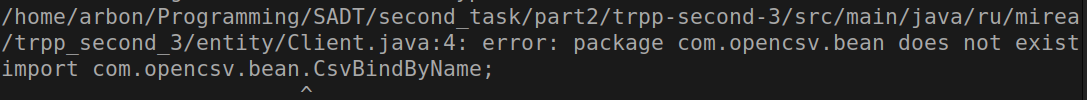
\includegraphics[width=0.7\textwidth]{Screenshot from 2023-03-12 18-05-52.png}
	\caption{Ошибка зависимоти}
	\label{fig:gradle:dep:undisc:error}
\end{figure}

Поэтому файл build.gradle была изменен как показано
на рисунке~\ref{fig:gradle:dep:undisc:good}.

\begin{figure}[h!tp]
	\centering
	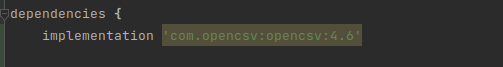
\includegraphics[width=0.8\textwidth]{Screenshot from 2023-03-12 17-25-18.png}
	\caption{Устраниение ошибки зависимости}
	\label{fig:gradle:dep:undisc:good}
\end{figure}

\paragraph{В некоторых классах поправить имя пакета}\mbox{}\par
При попытке собрать проект, командой: \texttt{./gradlew~build},
в файле ClientController были обнаружены не импортируемые пакеты.
Сообщение об ошибке показано на рисунке~\ref{fig:gradle:imp:error}.
Поэтому в соответствующие файлы были внесены необходимые строки.

\begin{figure}[h!tp]
	\centering
	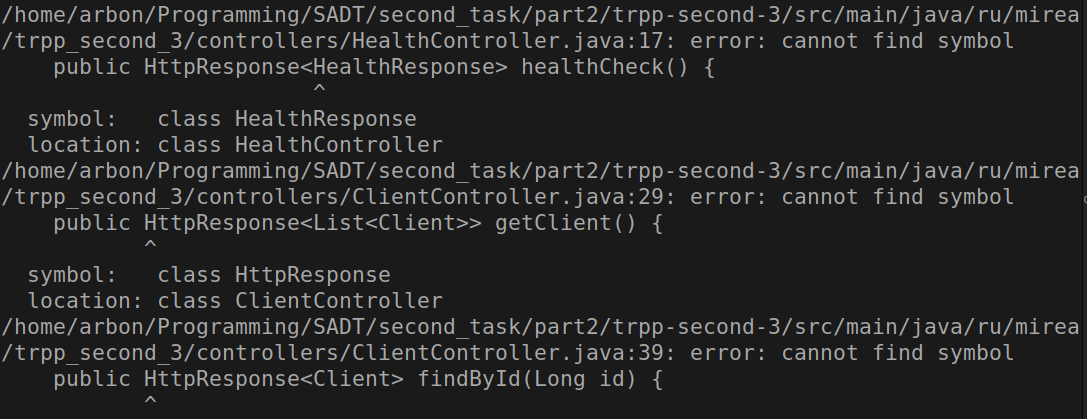
\includegraphics[width=0.8\textwidth]{Screenshot from 2023-03-12 18-16-05.png}
	\caption{Ошибки не омпортируемых пакетов}
	\label{fig:gradle:imp:error}
\end{figure}

А также необходимо исправить имя пакета в файле build.gradle, как показано
на рисунке~\ref{fig:gradle:build:pack}.

\begin{figure}[h!tp]
	\centering
	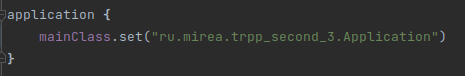
\includegraphics[width=0.8\textwidth]{Screenshot from 2023-03-12 19-08-52.png}
	\caption{Исправление пакет в build.grable}
	\label{fig:gradle:build:pack}
\end{figure}
\paragraph{Собрать документацию проекта, найти в ней запросы состояния
и сущности по идентификатору}\mbox{}\par
Для создания документации использовалась команда: \texttt{./gradlew~javadoc}.
Сгенерированая документация появиться в каталоге gradle/docs.
Пример сгенерированной документации показан
на рисунке~\ref{fig:gradle:javadoc}.

\begin{figure}[h!tp]
	\centering
	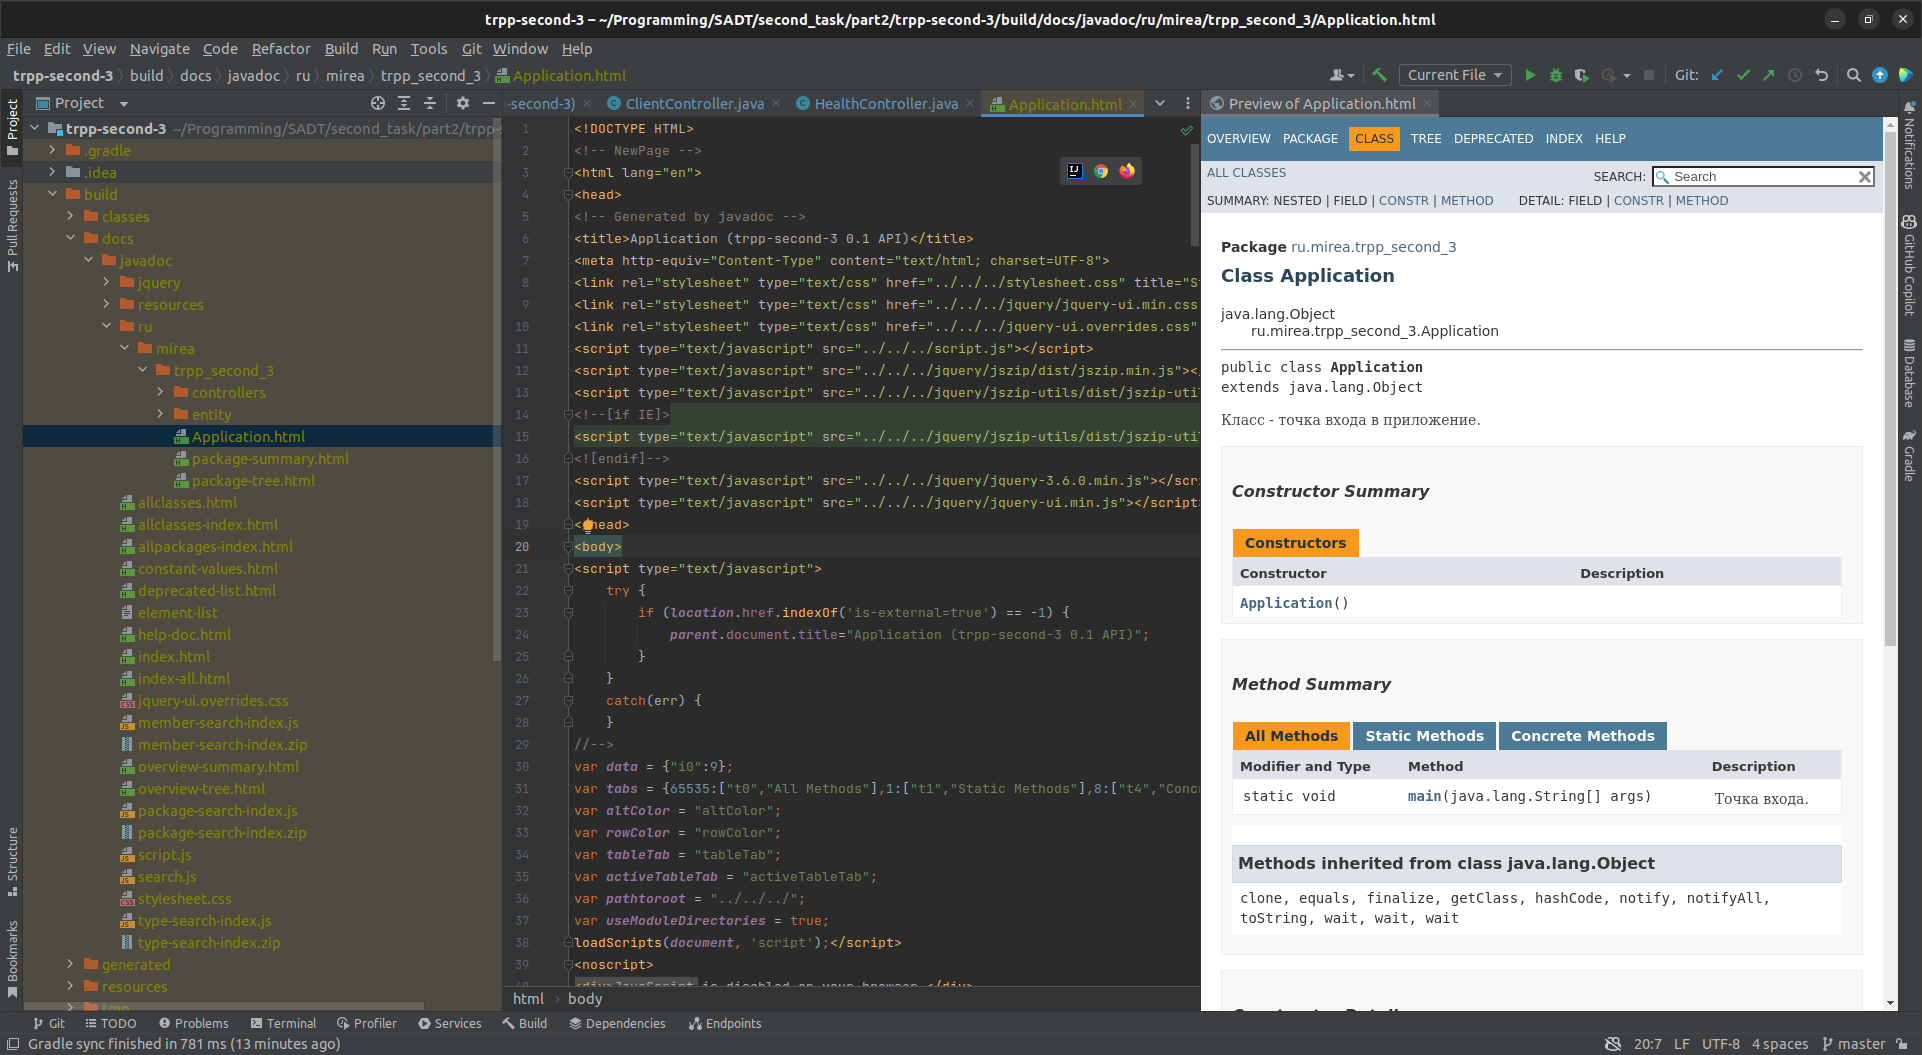
\includegraphics[width=0.8\textwidth]{Screenshot from 2023-03-12 18-27-47.png}
	\caption{Сгенерированая документация}
	\label{fig:gradle:javadoc}
\end{figure}

\paragraph{Собрать jar со всеми зависимостями (так называемый UberJar),
после чего запустить приложение. По умолчанию,
сервер стартует на порту 8080}\mbox{}\par
Для генерации jar понадобилась команда \texttt{./gradlew shadowJar},
которая собрает UberJar (архив со всеми зависимостями)
Для запуска приложения используется команда: \texttt{./gradlew run}
(Рисунок~\ref{fig:gradle:run}).

\begin{figure}[h!tp]
	\centering
	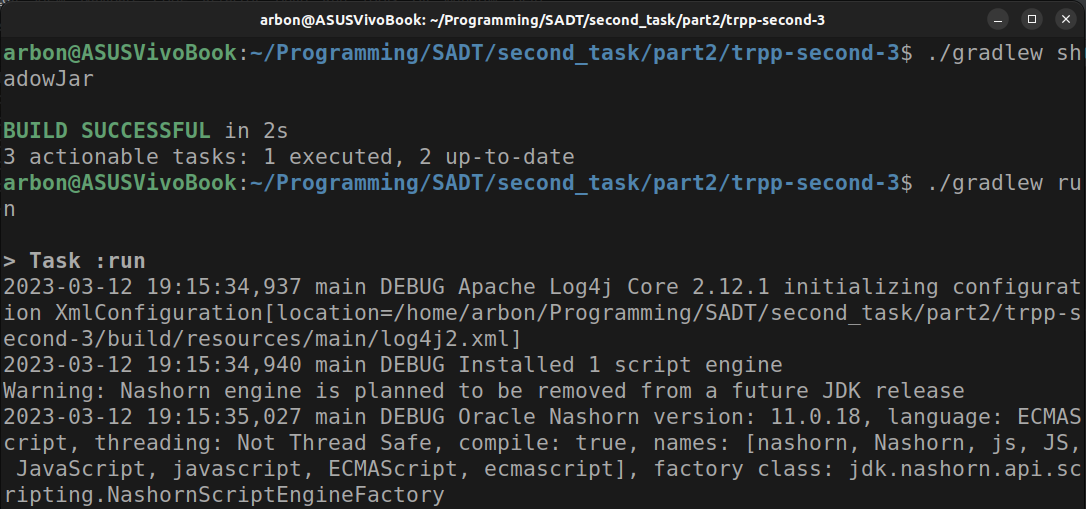
\includegraphics[width=0.8\textwidth]{Screenshot from 2023-03-12 19-16-01.png}
	\caption{Сборка jar и запуск приложения}
	\label{fig:gradle:run}
\end{figure}

\paragraph{Запросить состояние запущенного сервера
(GET запрос по адресу http://localhost:8080)}\mbox{}\par
Получить (GET) страницу в Linux можно с помощью команды: \texttt{curl}.
Вывод команды показан на рисунке~\ref{fig:curl}.

\begin{figure}[h!tp]
	\centering
	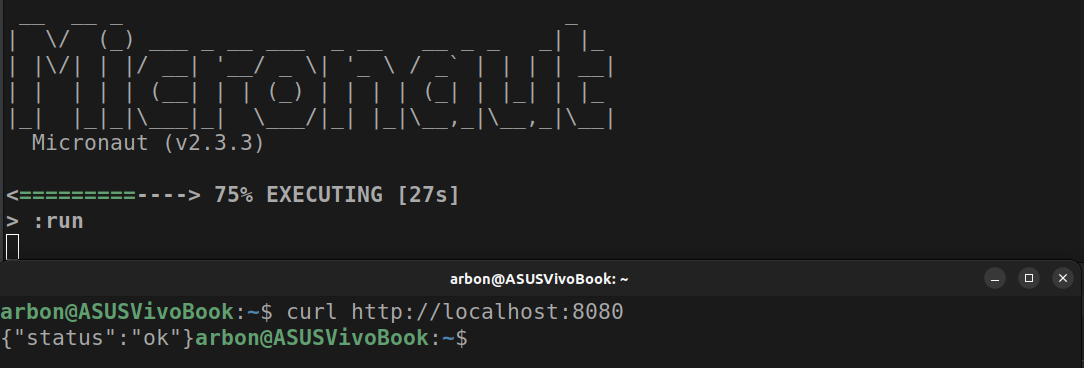
\includegraphics[width=0.8\textwidth]{Screenshot from 2023-03-12 19-51-03.png}
	\caption{GET запрос}
	\label{fig:curl}
\end{figure}

\paragraph{Запросить сущность по идентификатору
(GET запрос по адресу: http://localhost:8080/сущность/идентификатор)
Идентификатором будут 3 последних цифры в серийном номере вашего
студенческого билета.}\mbox{}\par
Аналогично примеру выше использовали каманду \texttt{curl},
передав параметром путь \textit{http://localhost:8080/client/874}.

\begin{figure}[h!tp]
	\centering
	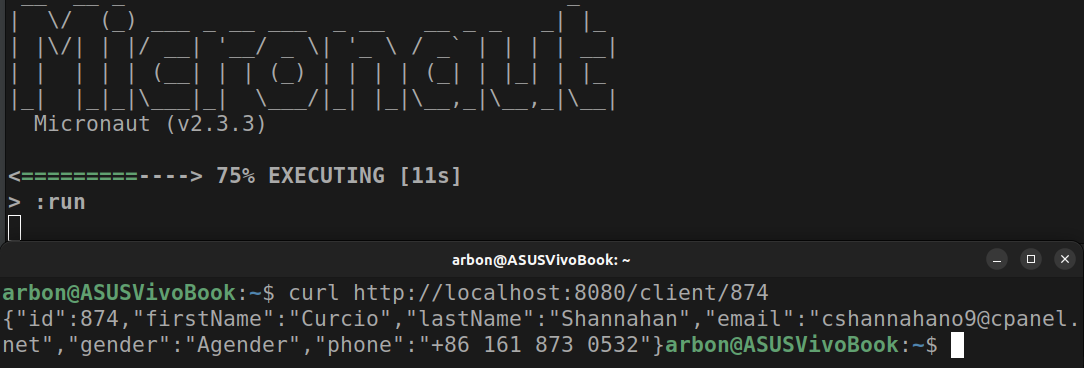
\includegraphics[width=0.8\textwidth]{Screenshot from 2023-03-12 20-08-05.png}
	\caption{GET запрос}
	\label{fig:curl:d}
\end{figure}

\paragraph{В задаче shadowJar добавить к jar-файлу вашу фамилию}\mbox{}\par
Чтобы добавить к jar-файлу текст нужно изменить файл build.gradle, как
показано на рисунке~\ref{fig:jar:rename}

\begin{figure}[h!tp]
	\centering
	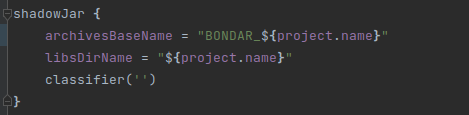
\includegraphics[width=0.8\textwidth]{Screenshot from 2023-03-12 20-32-59.png}
	\caption{Измененный build.gradle}
	\label{fig:jar:rename}
\end{figure}

Теперь после генерации в каталоге build/<имя проекта>/ появиться jar-файл
(Рисунок \ref{fig:jar:file}).

\begin{figure}[h!tp]
	\centering
	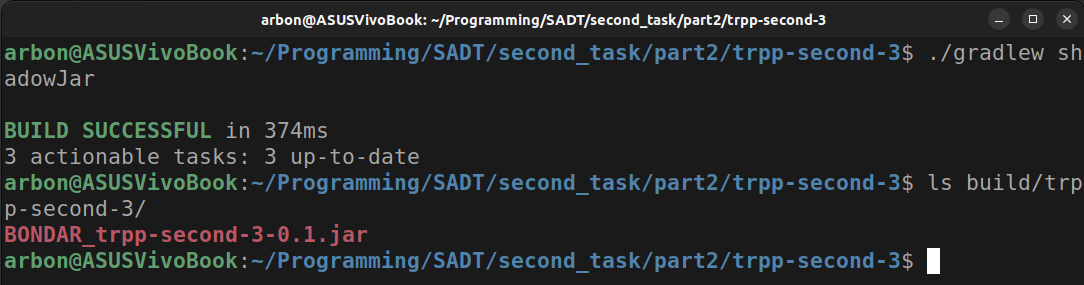
\includegraphics[width=0.8\textwidth]{Screenshot from 2023-03-12 20-32-42.png}
	\caption{Jar-файл}
	\label{fig:jar:file}
\end{figure}

\paragraph{Выполнить задачу checkstyleMain. Посмотреть сгенерированный отчет.
Устранить ошибки оформления кода.}\mbox{}\par

